% Chapter 1

\chapter{DIAGRAMAS DE FASE} % Main chapter title

(paper Shuiyao Huang et al. 2019) 



Most of these
gas particles lie on a well-defined curve in the phase diagram,
which is established by a balance between adiabatic cooling and photoionization heating. A fraction of gas particles are shock heated
when they collapse into the gravitational potential of dark matter
sheets and filaments and are driven into warm-and-hot ionized gas
outside of haloes (upper left) or fall into dark matter haloes and
become hot halo gas (upper right). Radiative cooling later plays a
critical role in the further condensation of gas into the condensed
region (lower right) where SF can occur. In addition, some gas goes
straight from the diffuse to the condensed region, i.e. cold mode
accretion (Keres et al. ˇ 2005, 2009a).



Calcule las fracciones al estilo de Martizzi 2009 y me dio, corte en dens = 2.5 y temp = 5 (la temperatura es el mismo corte, la densidad lo meti a ojo) Me dan muy diferentes. ESTO ES PARA EL VOID S
\begin{figure}[h]
\centering
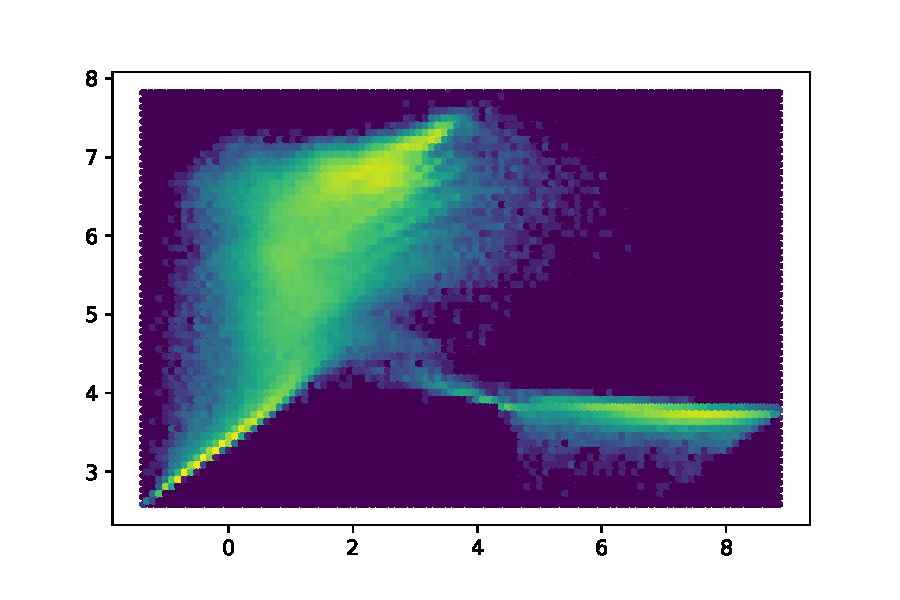
\includegraphics[width=14cm]{Figures/S1373_diagfaseVOID.pdf}
\decoRule
\caption[Diagrama de Fase TODAS particulas]{Densidad vs Temperatura considerando las particulas del void r<9.75}
\label{fig:Electron}
\end{figure}


fraccion DIF 0.19707932560856978

fraccion HALO 0.13583764565477252

fraccion WHIM 0.49660098890788423

fraccion WCGM 0.1704743649519073

fraccion SF 7.674876866194279e-06
\label{Chapter2} % For referencing the chapter elsewhere, use \ref{Chapter1} 

%----------------------------------------------------------------------------------------

% Define some commands to keep the formatting separated from the content 

%----------------------------------------------------------------------------------------
\section{R1198}

\begin{figure}[h]
\centering
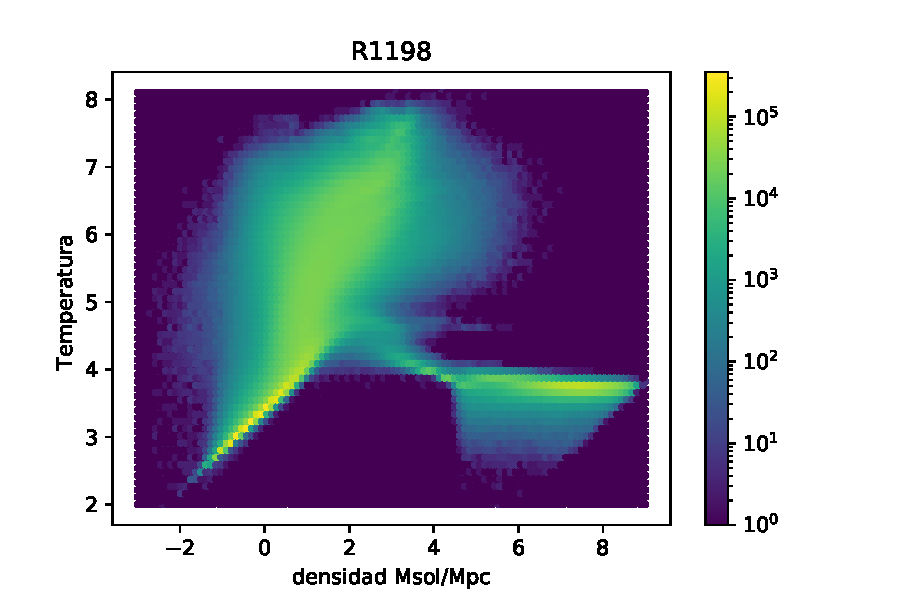
\includegraphics[width=18cm]{Figures/R1198_diagfase.pdf}
\decoRule
\caption[Diagrama de Fase TODAS particulas]{Densidad vs Temperatura considerando todas las particulas $\sim$ 33 millones}
\label{fig:Electron}
\end{figure}

\begin{figure}[h]
\centering
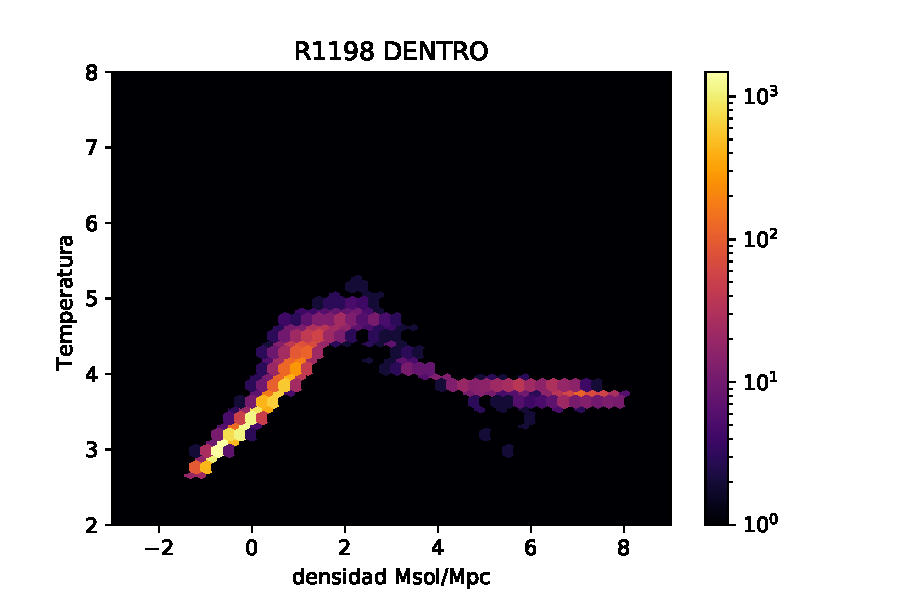
\includegraphics[width=18cm]{Figures/R1198_diagfase_int.pdf}
\decoRule
\caption[Diagrama de Fase R internas]{particulas dentro de un radio de 6 mpc}
\label{fig:Electron}
\end{figure}
\begin{figure}[h]
\centering
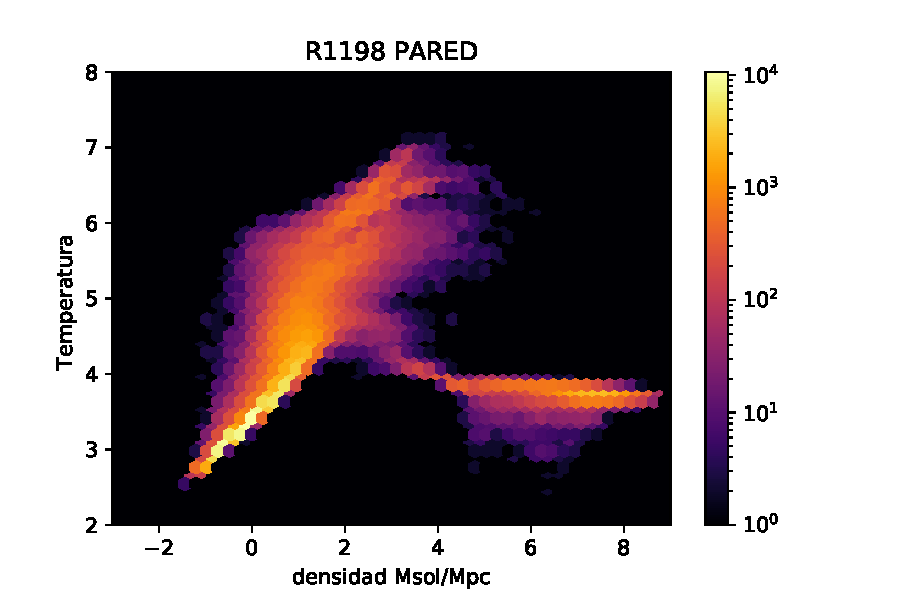
\includegraphics[width=18cm]{Figures/R1198_diagfase_wll.pdf}
\decoRule
\caption[Diagrama de Fase R pared]{particulas entre 6 y 12 Mpc}
\label{fig:Electron}
\end{figure}
\begin{figure}[h]
\centering
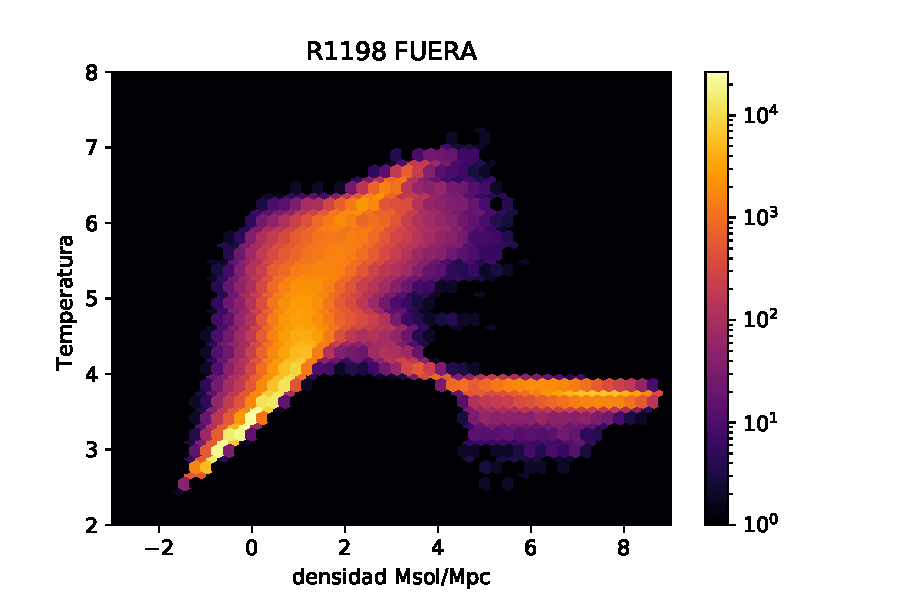
\includegraphics[width=18cm]{Figures/R1198_diagfase_ext.pdf}
\decoRule
\caption[Diagrama de Fase R externas]{particulas entre 12 y 18 Mpc}
\label{fig:Electron}
\end{figure}




\section{S1373}

\begin{figure}[h]
\centering
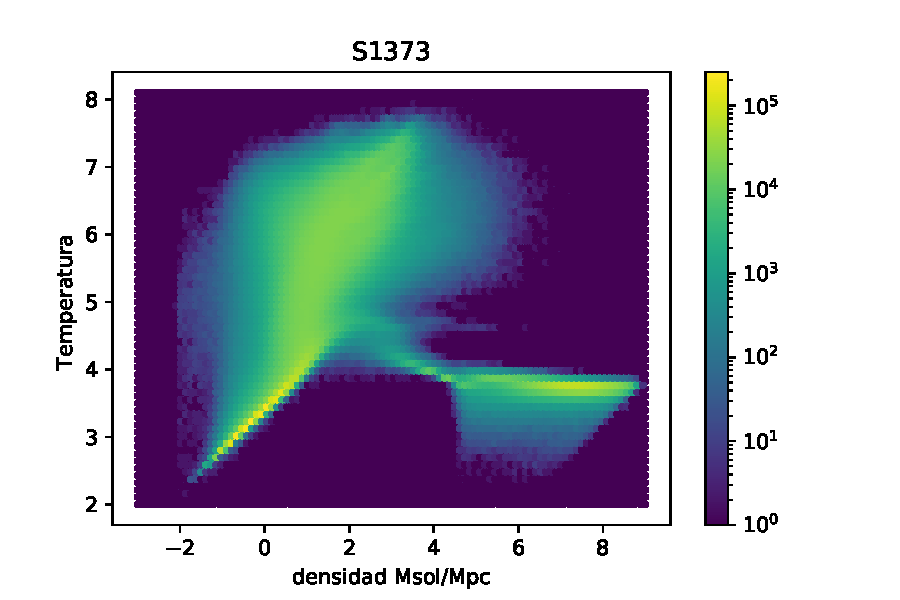
\includegraphics[width=18cm]{Figures/S1373_diagfase.pdf}
\decoRule
\caption[Diagrama de Fase TODAS particulas]{Densidad vs Temperatura considerando todas las particulas $\sim$ 33 millones}
\label{fig:Electron}
\end{figure}



\begin{figure}[h]
\centering
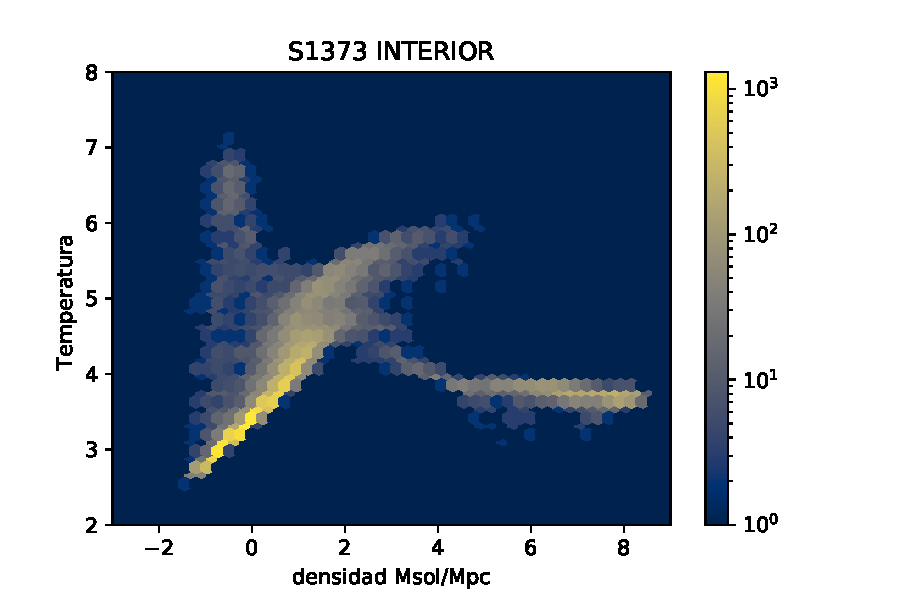
\includegraphics[width=18cm]{Figures/S1373_diagfase_int.pdf}
\decoRule
\caption[Diagrama de Fase S internas]{particulas dentro de un radio de 6 mpc}
\label{fig:Electron}
\end{figure}
\begin{figure}[h]
\centering
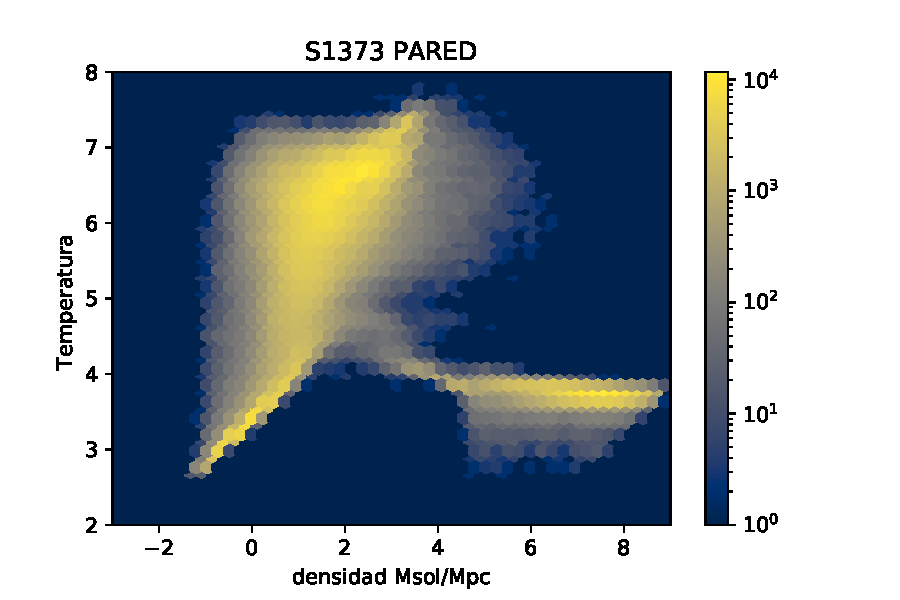
\includegraphics[width=18cm]{Figures/S1373_diagfase_wll.pdf}
\decoRule
\caption[Diagrama de Fase S pared]{particulas entre 6 y 12 Mpc}
\label{fig:Electron}
\end{figure}
\begin{figure}[h]
\centering
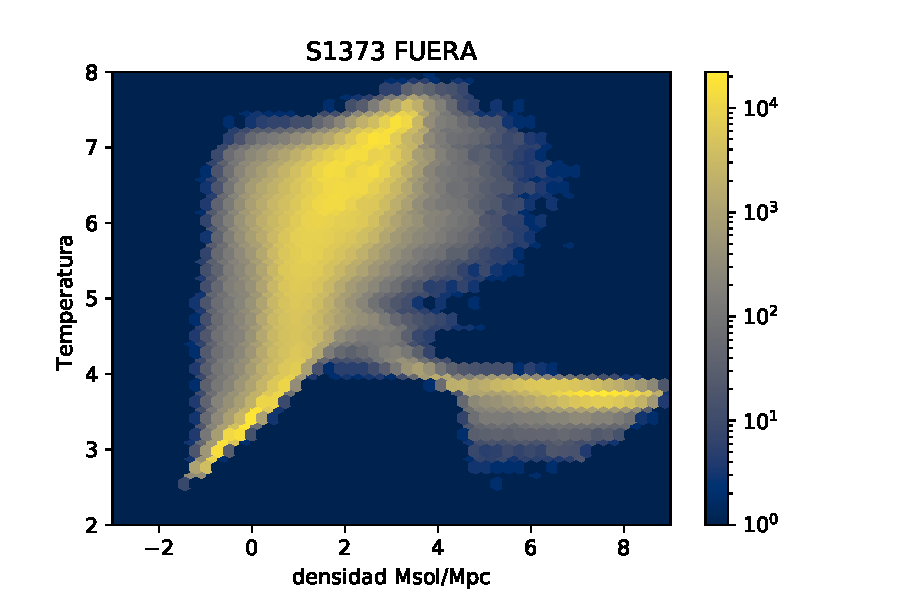
\includegraphics[width=18cm]{Figures/S1373_diagfase_ext.pdf}
\decoRule
\caption[Diagrama de Fase S externas]{particulas entre 12 y 18 Mpc}
\label{fig:Electron}
\end{figure}